\chapter{Metodología y desarrollo}

\section{Consideraciones generales previas al desarrollo}

Para el desarrollo de nuestro trabajo definimos al empezar una serie de hitos que debian cumplirse de forma secuencial. De forma que al cumplirse todos tendriamos una herramienta que cumpliria con la especificación que hemos definido en la introducción. La lista de esos objetivos es la siguiente

\begin{enumerate}
\item Renderizado eficiente de una malla 3D con una cantidad elevada de poligonos
\item Implementación de una camara controlable por el usuario que permita examinar la malla 3D
\item Poder extraer información sobre la profundidad de la malla 3D desde nuestra perspectiva
\item Poder hacer identificable la información extraida sobre la profundidad a nivel de estructura de la malla
\item Diseño de un Algoritmo capaz de detectar la presencia de convexidades en la malla desde nuestra perspectiva
\item Implementar una forma de visualizar y controlar de forma interactiva las transformaciones sobre la convexidad detectada
\item Capacidad de exportar la malla transformada a un formato de descripción de objetos tridimensionales
\end{enumerate}

Una vez definimos esta hoja de ruta del proyecto el siguiente paso fue decidir la tecnología exacta en la que se implementaria el proyecto, ademas de si se utilizaría o no alguna utilidad que permitiera abstraer a un nivel mas alto el uso de graficos en el trabajo. En primer lugar la decision radico entonces entre utilizar OpenGL o Web
GL como API de graficos, en caso de utilizar WebGL el proyecto utilizaria un stack de tecnología web, utilizando principalmente Javascript y Three.js para gestionar la parte de graficos. Mientras que si usabamos OpenGL usariamos C++ y tendriamos que investigar si utilizar simplemente un gestor de ventanas o si por el contrario podriamos utilizar
algun framework de desarrollo de aplicaciones con graficos tridimensionales que nos ofrezca una abstracción similar a la que nos da Three.js. La decisión final fue la de utilizar OpenGL sobre WebGL. Esto se decidio así por varias razones. La primera y principal es que OpenGL es mucho mas flexible y esta mas optimizado que WebGL.
Esto ocurre porque WebGL esta basado en OpenGL ES 2.0, una versión de OpenGL simplificada diseñada especificamente para crear un estandar de gráficos más simplificado que OpenGL para dispositivos moviles. WebGL ademas de eso esta diseñado para ejecutarse principalmente en Navegadores, lo cual añade limitaciones propias sobre las que OpenGL ES presenta. Por otro lado, el proyecto debe estar capacitado para lidiar con
esculturas complejas que presenten un gran numero de poligonos sobre los cuales ademas deberemos operar. Esto hace que utilizar un lenguaje compilado como C++ sobre otro interpretado como Javascript ganara fuerza. Por tanto la decisión final fue la de utilizar OpenGL como API de graficos y utilizar C++ como lenguaje en el que se desarrollaria el proyecto.



El siguiente punto fue decidir si ibamos a utilizar solo un gestor de ventanas minimo y las llamadas de OpenGL o si ibamos a utilizar algun framework para desarrollar aplicacions de C++ que incluyera utilidades graficas. Durante este periodo se considero el uso de OpenFrameworks para realizar el proyecto.



OpenFrameworks es un framework de experimentación para C++ que trata de ser una herramienta de uso general. Agrupando diferentes librerias usadas en C++ para ofrecer una caja de herramientas que permita desarrollar aplicaciones capaces de utilizar capacidades como los graficos por ordenador, la vision por computador, la carga de modelos 3D de forma transparente y sencilla para el usuario. \cite{openframeworksAboutOpenFrameworks}
Al principio del desarrollo decidimos utilizarlo para realizar experimentación con el lenguaje de Shaders de GLSL de forma sencilla. Siguiendo ademas la recomendación que el libro \cite{Halladay2019-xi} que utilizamos para aprender a usar GLSL nos ofrecio.

Tras pasar una semana probando la herramienta finalmente decidimos descartarla, la razón de esto fue que aunque la herramienta ofrecia muchas comodidades para realizar tareas sencillas de graficos
el desarrollo de la aplicacion iba a requerir el uso de conceptos mucho mas avanzados de graficos para los cuales apenas habia documentación sobre como implementar o usar utilizando la libreria. Mientras que por otra parte encontramos una buena cantidad de documentación y ejemplos sobre como implementar los conceptos que requeriamos para nuestro empeño usando simplemente la API de OpenGL.

Por tanto tras este periodo de experimentación se decidio que 
implementariamos nuestro proyecto sin utilizar ningun framework. Partiendo del material desarrollado por el tutor Francisco Javier Melero Rus para la realización de las practicas de la asignatura de Informática Gráfica. Este material consta de la base para comenzar un proyecto de graficos por ordenador y esta liberada bajo la licencia GPL\cite{gplv3}.

La plantilla incluye una clase que gestiona el uso de GLUT para la creación y gestion de ventanas. GLUT es una lirbreria creada con la idea de simplificar el uso de OpenGL aportando una serie de utilidades, el funcionamiento de GLUT utiliza callbacks llamando a funciones cuando se dan ciertos eventos a los que esta atendiendo, como la pulsación de una tecla, el movimiento del raton, o el redimensionamiento de la ventana. Nosotros lo usamos principalmente para inicializar el contexto de OpenGL, crear una ventana de las dimensiones que le especifiquemos. Indicarle cual es la función de dibujado principal, Que funciones debe llamar ante los eventos de redimensionado, pulsación de una tecla, movimiento del raton y pulsación del raton e iniciar un bucle que efectua la función de dibujado de forma infinita.

Todo esto se realiza en la clase que contiene el matodo main del proyecto. Pero todas las funcionalidades del proyecto estan abstraidas en diferentes clases. Siendo la mas importante de todas la clase Escena que contiene el metodo de dibujado entre otros metodos tambien importantes.

Adicionalmente la plantilla incluye tambien la implementación de clases Tupla auxiliares utiles para cuando estemos trabajando con datos como vertices que han de expresarse como vectores de 3 coordenadas en el espacio tridimensional. Estas clases aunque utiles se ha limitado su uso en favor del uso de la biblioteca OpenGL Mathematics \cite{gtrucOpenGLMathematics}. O GLM para abreviar. Esta biblioteca distribuida bajo la licencia MIT \cite{GLMLICENSE} ofrece varias utilidades matematicas implementadas bajo el mismo nombre que las utilidades matematicas que ofrece GLSL. Esto permite que sea facil utilizar la libreria si conoces GLSL. Pero no se limita solo a eso, sino que tambien aporta una serie de utilidades como transformaciones matriciales que nos seran extremadamente utiles para el desarrollo del proyecto. Por tanto estas clases implementadas para esta plantilla han visto su uso ligeramente limitado en favor de las utilidades que nos daba GLM.

Una vez definido la base de nuestro trabajo podemos pasar a definir los diferentes elementos que hemos desarrollado en base a la consecución de los objetivos anteriormente definidos. Para despues de ello comentar la estructura general del proyecto.

\section{Renderizado de mallas 3D genericas con un alto numero de poligonos}

El primer paso para poder hacer nuestro proposito es ser capaz si quiera de renderizar una malla 3D. Para hacer esto en OpenGL es necesario especificarle tanto los vertices que forman parte de la malla como las caras definidas por estos vertices. Esto nos deja un único problema a la hora de definir la malla, que es la orientación de los triangulos. Aun siendo una primitiva plana hay que definir cual es la cara frontal de un triangulo y cual es la cara trasera. Por convención se define la cara delantera de un triangulo segun la especificación de los vertices. De forma que la cara en la que los vertices estan en sentido antihorario en el orden en el que se han declarado se considera la cara delantera del triangulo.

\begin{figure}
\centering
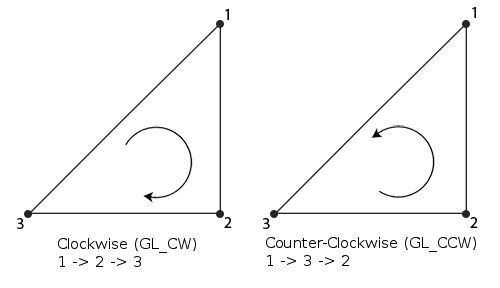
\includegraphics[scale=0.5]{imagenes/Winding_order.png}
\caption[Definicion de un triangulo]{Variación a la hora de definir un triangulo, la cara delantera es aquella que se define con los vertices en el sentido antihorario}

\end{figure}

En la especificación 1.0 de OpenGL Cada vertice tenia que declarse de forma manual con una instrucción especifica para definirlo. Sin embargo a partir de OpenGL 2.0 Se utilizan buffers para almacenar toda la información de la malla, sea vertices, normales, caras o coordenadas de texturas en diferentes buffers. Luego estos se envian a la tarjeta grafica de una sola vez utilizando la orden de OpenGL correspondiente. De forma normal en cada frame de dibujado se envia de vuelta toda la información a la GPU. Esto es lo que se conoce como modo directo de dibujado. Sin embargo, hay una forma mas eficiente de gestionar esto. Lo cual considerando la necesidad de renderizar mallas detalladas con un alto numero de poligonos
es mejor enviar solo una vez la información. Dejarla almacenada en la memoria de la GPU. Crear algun medio por el cual referenciar esa información y en cada frame de dibujado solo se le dice a la grafica que utilice la información referenciada. Esto permite mejorar el rendimiento y es la forma moderna estandar de trabajar en OpenGL puesto que ahorra transferencias innecesarias de datos. Para poder hacer esto utilizamos lo que se conoce como un Vertex Buffer Object o VBO, lo cual no es mas que un bloque de memoria contigua en GPU \cite{khronosVertexSpecification} Con este mecanismo conseguimos apurar un poco más el rendimiento.

Sabiendo que hemos usado eso hemos creado una clase Malla3D abstracta que gestiona todo el dibujado. Y finalmente como todos los modelos que vamos a trabajar van a estar importados desde archivo. Concretamente y por simplicidad vamos a limitar los archivos que podemos abrir a archivos de formato .Ply este formato describe una malla 3D de una forma sencilla, contando con una cabecera con información relevante para su lectura y toda la información que describe la malla puesta linea a linea. Para leer estos archivos hemos utilizado unas funciones escritas por el profesor de la UGR Carlos Ureña y liberado bajo la licencia GLP \cite{gplv3}.
Finalmente creamos una clase que herede de la clase Malla3D que en su constructor utilizara esas funciones de lectura para extraer la información del archivo y utilizar luego los metodos de Malla3D para gestionar el dibujado.

\begin{figure}
\centering
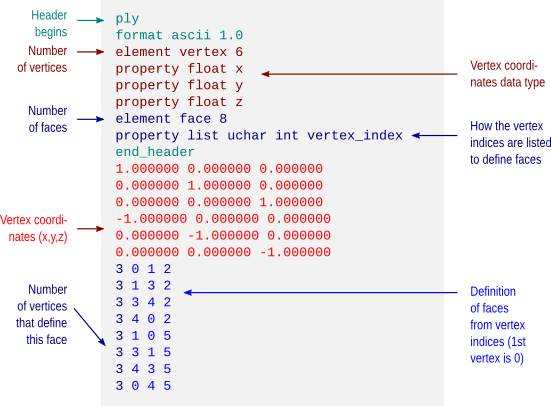
\includegraphics{imagenes/format-ply.png}
\caption{Funcionamiento del formato .ply}

\end{figure}

\section{Implementación de una Camara controlable por el usuario}

Despues de ser capaces de renderizar la malla necesitamos ser capaces de poder visualizarla desde diferentes puntos de vista. Para ello necesitamos definir una camara que ademas deberemos ser capaces de controlar de forma interactiva.

Para definir una camara necesitamos establecer su posición en el espacio y su orientación. Para ello se definen dos puntos en el espacio. El punto eye que representa el lugar del espacio en el que se encuentra colocada la camara y el punto at que representa el lugar del espacio hacia el que la camara esta mirando.
Esto sin embargo no es suficiente para definir una camara. Pues aunque sabemos donde estamos y que estamos mirando nos falta saber una información relevante. Como lo estamos mirando. No es lo mismo la forma en la que se vera un objeto si estamos cabeza arriba o si estamos cabeza abajo. Para ello definimos un ultimo elemento,
el vector Up, que indica donde esta el arriba. 

Con estos elementos podemos definir la matriz de vista que hemos mencionado en la introducción. Para ello primero definimos un nuevo sistema de coordenadas que nos define la camara. Para ello vamos a calcular 3 vectores.

\begin{list}{.}{}
\item El primer vector vamos a llamarlo Z ya que definira el eje Z de nuestro nuevo sistema de coordenadas. Este vector
se computa de la siguinte forma $\hat{Z}=(\frac{({at}-{eye})}{|({at}-{eye})|})$ Es decir, el vector normalizado resultante de restar el punto at al punto eye
\item El siguiente vector lo llamaremos X, ya que nos definira el eje X de nuestro nuevo sistema de coordenadas, viene a representar lo que esta a la derecha de la camara. Para obtener este vector sabemos que el vector que esta a la derecha deberia ser perpendicular al vector que indica la dirección de que esta arriba y a este vector Z
que hemos calculado que representa lo que hay delante. Por tanto lo calculamos de la siguiente manera $\hat{X}=(\frac{(\vec{up} \times \vec{Z})}{|(\vec{up} \times \vec{Z})|})$ Es decir, el vector normalizado fruto de calcular el producto vectorial entre el vector Up y el vector Z calculado anteriormente.
\item Finalmente un vector al que llamaremos Y que nos definira la dirección hacia arriba en nuestro nuevo sistema de coordenadas. No puede ser el Up porque no tenemos garantias que sea perpendicular a nuestros vectores Z y X, por tanto tenemos que recalcularlo. Para ello simplemente lo calculamos de la siguiente forma $\hat{Y}=\frac{(\vec{X} \times \vec{Z})}{|(\vec{X} \times \vec{Z})|}$ Esto es, el vector normalizado perpendicular al vector X y Z que hemos calculado antes
\end{list}

Con estos tres vectores y la posición de la camara podemos calcular una matriz de vista que permita convertir un punto en las coordenadas de mundo a un punto en el nuevo sistema de coordenadas que hemos definido por la camara. Para construir este punto. Esta matriz se calcula de la siguiente forma \cite{learnopenglLearnOpenGLCamera}

$$ {View}=  \begin{pmatrix}
    X.x & X.y & X.z & 0.0 \\
    Y.x & Y.y & Y.z & 0.0 \\
    Z.x & Z.y & Z.z & 0.0 \\
    0.0 & 0.0 & 0.0 & 1.0 
    \end{pmatrix} *  \begin{pmatrix}
        1.0 & 0.0 & 0.0 & {eye.x} \\
        0.0 & 1.0 & 0.0 & {eye.y} \\
        0.0 & 0.0 & 1.0 & {eye.z} \\
        0.0 & 0.0 & 0.0 & 1.0 
        \end{pmatrix}  $$ 

Por suerte la libreria de OpenGL Mathematics nos hace el trabajo y nos calcula esta matriz de forma automatica con su función LookAt a partir de los parametros de la camara que hemos definido. Esto nos permite calcular la matriz de vista de forma facil.

Por otra parte como ya dijimos previamente la matriz de vista no es la unica transformación. Recordemos tambien que tenemos que calcular las transformaciones propias de la proyección. Para ello tenemos que calcular la matriz de proyección de la que hablamos en la introducción.

Para este proyecto hemos utilizado una proyección en perspectiva que inmita el funcionamiento de la vista humana. La forma de utilizar esta perspectiva es definir una piramide truncada de base rectangular o Frustrum que servira para definir la camara.
sobre esta piramide truncada definimos dos planos, de forma que todo lo que quede dentro de esos dos planos sera renderizado por la camara. Estos dos planos se definen con dos valores numericos que simbolizan la distancia a la posición de la camara.
Estos dos valores se denominan near y far. Todo lo que quede por delante del near o por detras del far no sera renderizado y no estara visible Finalmente hay que especificar lo ancha que es esa piramide de base rectangular. Para ello tenemos 4 parametros
top, right, left y bottom que nos ayudan a denominar el tamaño de la base de la piramide.

De estos parametros podemos construir la matriz de proyección de la siguiente manera \cite{ibmGlFrustumSubroutine}

$$ {Projection}=  \begin{pmatrix}
    \frac{2*{Near}}{{Right}-{left}} & 0 & \frac{{Right}+{Left}}{{Right}-{Left}} & 0.0 \\
    0.0 & \frac{2*{Near}}{{Top}-{Bottom}} & \frac{{Top}+{Bottom}}{{Top}-{Bottom}} & 0.0 \\
    0.0 & 0.0 & \frac{{Far}+{Near}}{{Far}-{Near}} & \frac{2*{Far}*{Near}}{{Far}-{Near}} \\
    0.0 & 0.0 & -1.0 & 0.0 
    \end{pmatrix} $$

Igual que con la matriz de vista, tenemos una utilidad de OpenGl Mathematics que nos calcula esta matriz de forma automática.

La clase camara que hemos implementada se encarga de gestionar y darnos las matrices de vista y proyeccion. Al estar usando la pipeline de graficos programable no podemos contar con que OpenGL haga las transformaciones de forma automatica.
Necesitamos pasarle a nuestro vertex shader la matriz de modelo vista proyección. No hemos mencionado como se calcula la matriz de modelo. Pero en esencia es una matriz unitaria a la que vamos multiplicando las diferetes transformaciones 
que queremos aplicar sobre nuestro modelo.

La matriz modelo vista proyección es el resultado de multiplicar las tres matrices. Recordemos que la multiplicación de matrices no respeta la propiedad conmutativa. Por tanto tenemos que multiplicar las matrices a la izquierda para ir aplicando las transformaciones en orden.
En el vertex shader multiplicamos cada vertice por esta matriz y esa sera la posición final del vertice.

Para la parte de que el usuario pueda controlar la camara aprovechamos el teclado y el raton. Mencionamos antes que teniamos una función que gestionaba las pulsaciones de teclado y los movimientos del raton.
En esa función podemos ir actualizando los valores de la camara en función de las teclas que pulsamos. Ademas también es conveniente que podamos controlar la camara de varias formas. En nuestro caso hemos planteado el movimiento de la camara
de dos maneras, un modo fijo donde el at esta fijado al origen de coordenadas y el eye es lo que se mueve. Y otro modo libre donde el eye esta fijo y el at es lo que se mueve



\begin{figure}
    \centering
    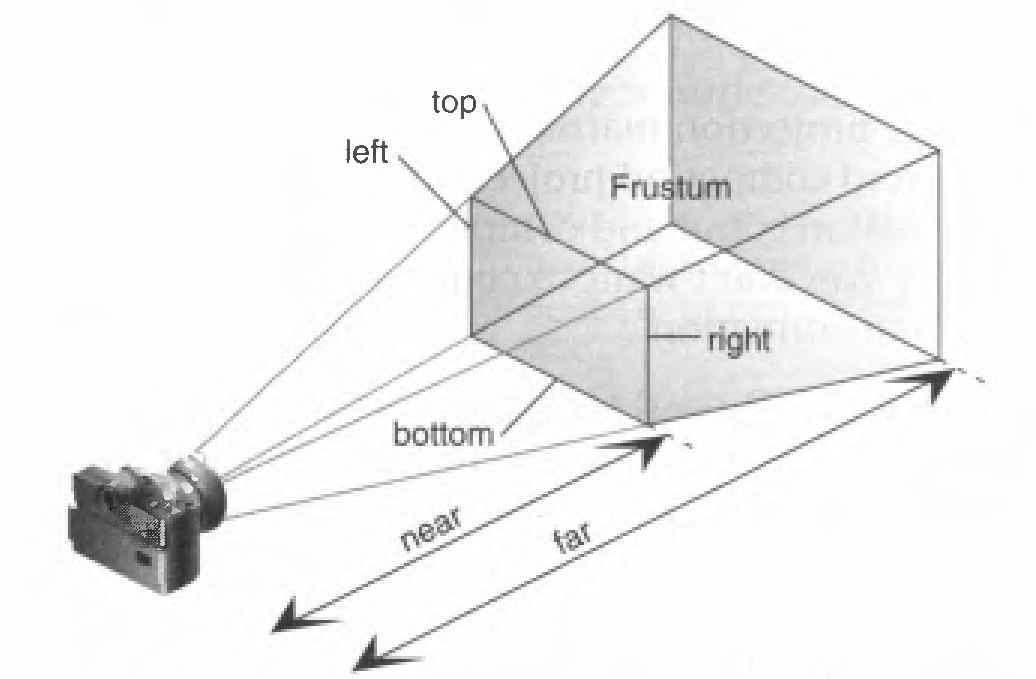
\includegraphics{imagenes/frustrum.png}
    \caption{Visualización de los parametros de proyección}
\end{figure}




\section{Extracción de información sobre la profundidad de la malla 3D}

Ya contamos con una camara funcional y podemos renderizar los modelos que queramos. Ya estamos juntando todos los componentes que nos hacen falta. Sin embargo aun necesitamos una ultima cosa para empezar. Necesitamos algun metodo para conocer el valor de profundidad de lo que estamos viendo. De forma ideal nos interesaria conocer el valor de profundidad de un vertice. Sin embargo no tenemos ningun mecanismo que nos de esto de forma directo. Aun así contamos con un recurso vital en graficos por ordenador que nos permite conocer
un valor de profundidad para un pixel concreto. Este metodo es lo que se conoce como el algoritmo de Z-buffering. La razón por la que este algoritmo se invento es por la necesidad de determinar que primitivas renderizar y cuales no. Esto es importante ya que si tenemos por ejemplo dos figuras renderizadas una detras de otra en escena debemos saber que valor de color darle a los pixeles que podrian pertenecer a una figura o a otra. Dandole siempre el valor de color correspondiente al de la figura con menor profundidad de las dos.

Para esto OpenGL de forma interna utiliza un buffer del tamaño del numero de pixeles de la pantalla con todos sus elementos inicializados a un valor maximo de 1. Antes hablamos de que cuando se calculan fragmentos un pixel puede tener mas de un fragmento posible. Este es un caso donde eso ocurre. Por cada elemento dibujado en escena el cual ese pixel podria renderizar se genera un fragmento. Este fragmento contiene información de profundidad. Este valor se calcula a partir de la profundidad real de ese fragmento y pasa por una serie de transformaciones
hasta acabar en un valor dentro del intervalo $[0,1]$ donde un valor de 0 representa que ese fragmento esta exactamente en el near de la camara y un valor de 1 representa que esta exactamente en el far de la camara.

Por cada fragmento calculado se comprueba su profundidad y si es menor que el valor del buffer de profundidad del pixel correspondiente se actualiza el valor del buffer de profundidad. OpenGL renderizara por defecto el pixel con el valor de color del fragmento con menor valor de profundidad para cada pixel. \cite{javatpointComputerGraphics}

\begin{figure}
\centering
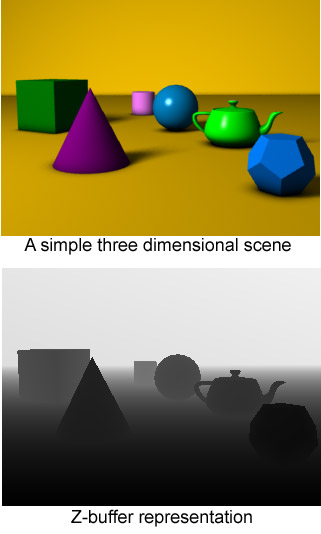
\includegraphics{imagenes/Z-buffer.jpg}
\caption[Visualización del Z-buffer]{Visualización del Z-buffer, los valores mas cercanos al near de la camara se ven mas oscuros porque tienen un valor de z-buffer mas cercano a 0, mientras que cuanto mas nos alejamos se ve de un color mas blanco}

\end{figure}

Ademas de ser muy util para openGL este buffer de profundidad final es vital para nuestro algoritmo. Pues nos permite tener una idea de la profundidad de lo que estaos visualizando con respecto la camara. Así que es importante que podamos leer de el. Sin embargo este buffer no es accesible de forma directa en la CPU puesto que todos estos calculos se realizan en la GPU durante el pipeline de graficos. Por tanto necesitamos un mecanismo para poder acceder a esta información. Para ello necesitamos afinar un concepto sobre como se generan las imagenes en pantalla.
hasta ahora asumiamos que OpenGL renderizaba siempre en pantalla. Sin embargo realmente esto no tiene porque ser así. OpenGL trabaja con lo que se conoce como framebuffers. Estos buffers son similares al Z-buffer que hemos descrito antes. Ambos son arrays que contienen tantos elementos como pixeles hay en pantalla. Solo que en el caso de los framebuffers en vez de contener información sobre la profundidad contienen información sobre el valor de color de cada pixel en concreto. Si no especificamos
OpenGL renderiza hacia un framebuffer y luego vuelca la información de ese framebuffer directamente en pantalla. Sin embargo gracias a un mecanismo introducido en OpenGL 3.0 llamado los frame buffer object podemos controlar a que framebuffer renderizamos y que hacemos con esa información. Los frame buffer object nos permiten renderizar objetos en escena y luego decidir que hacer con los diferentes buffers. Sea mandarlos a un objeto sobre el que luego no vamos a leer o mandarlos a una textura. En nuestro caso hemos decidido mandar tanto el buffer de profundidad como
el framebuffer como texturas. \cite{khronosFramebufferObject}

Para OpenGL una textura es realmente un array. En caso de las dos texturas que hemos guardado de tantos elementos como pixeles tenga la ventana donde el primer elemento corresponde con el pixel de la esquina inferior izquierda de la ventana. Una vez hemos renderizado la escena y hemos guardado la información de la profundidad y el color en las texturas vamos a hacer dos cosas. La primera es recuperar la información de los arrays de la textura utilizando la función pertinente de OpenGL. La segunda es resolver que hacer con el dibujado en pantalla. Como hemos renderizado la escena
en un framebuffer object distinto del framebuffer estandar de OpenGL todo lo que hemos dibujado no se esta renderizando por pantalla. Y si quisieramos visualizarlo tendriamos que volver a renderizar la escena entera. Sin embargo podemos aprovechar que hemos guardado la información del framebuffer en textura para permitirnos no volver a renderizarlo todo y en su lugar renderizar simplemente dos triangulos que formen un rectangulo del tamaño de la ventana. Esta figura geometrica se conoce como un Quad. Lo dibujamos en pantalla, de forma que ocupe siempre toda la vista y texturizamos el quad 
con la información del framebuffer de nuestro framebuffer Object. De este modo conseguimos la ilusión de que se esta renderizando otra vez la escena entera otra vez en el framebuffer de la pantalla cuando en su lugar se estan renderizando solamente dos triangulos. 

\begin{figure}
    \centering
    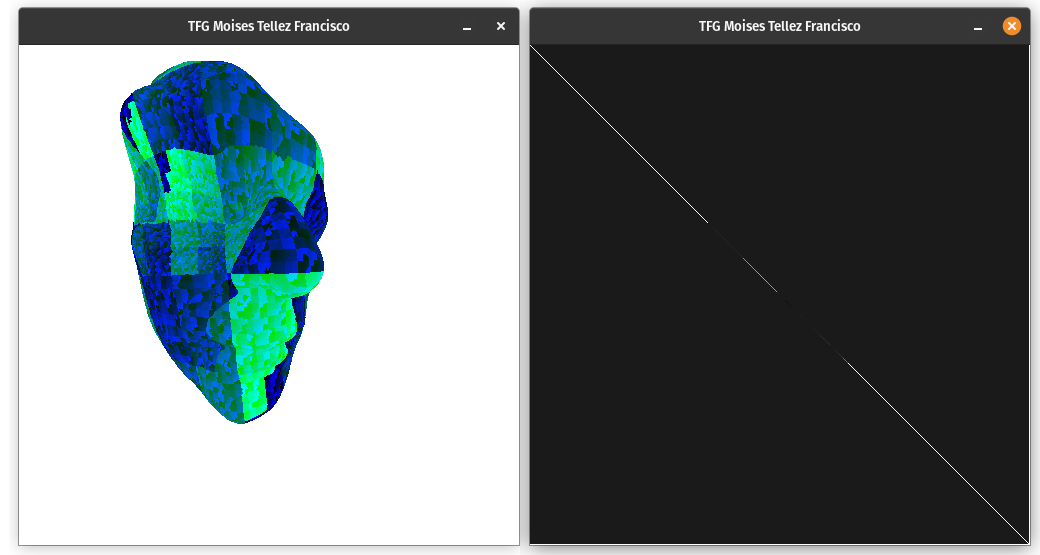
\includegraphics[scale=0.3]{imagenes/fbo.png}
    \caption[Renderizado de la información de un framebuffer Object]{Renderizado de la información del framebuffer Object en un Quad, a la izquierda se ve la escena si visualizamos el quad relleno con su textura mientras que a la derecha se ve la escena si solo dibujamos las lineas de los poligonos que la forman}
\end{figure}

\section{Identificación de la información extraida a nivel estructural de la malla}

Aunque ya tenemos la forma de acceder a la información sobre la profundidad de nuestro renderizado tenemos un problema que de cara al momento en que queramos transformar los triangulos despues de encontrar la convexidad. Y es el hecho de que toda esta información no se calcula a nivel de vertice. Sino que se hace a nivel de fragmento. No podemos conocer la profundidad de un vertice concreto. solo la de un pixel de la pantalla. Por tanto necesitamos alguna forma de poder traducir la iformación a nivel de fragmento a nivel de vertice o de triangulos. Para esto vamos a utilizar un recurso de GLSL que nos va a ser extremadamente util.
El fragment Shader tiene una variable a la que se puede acceder que se conoce como Gl\_PrimitiveID \cite{khronosGlPrimitiveIDOpenGL} Esta variable se calcula inicializando un contador a 0, y cada vez que se llama a la función de dibujado de una malla y se le pasa a OpenGL información sobre las primitivas que componen esa malla se incrementa en uno por cada primitiva que considera. De esta manera cada primitiva de la escena tiene un identificador unico y en el fragment Shader puedes saber que primitiva estas dibujando. Esto es especialmente esclarecedor en nuestro caso donde la unica cosa que estamos renderizando en escena es la malla
sobre la que queremos trabajar. Por tanto en nuestro caso la primera cara definida en la lista de caras tendra un id de primitiva de 0 y así de forma incremental con todas.
Sabiendo esto si conseguimos que cada primitiva tenga un color único y distinto de todas las demas podemos utilizar la textura con la información del color que hemos mencionado antes para conocer que primitiva estamos tratando, y como sabemos que el Id de primitiva es equivalente a la posición en el array de caras podemos también facilmente que vertices forman parte de esa primtiva.

Otro detalle interesante es que existe una variable equivalente en los vertex shaders llamada GL\_VertexID \cite{khronosGlVertexIDOpenGL}, la forma de calcularlo es equivalente pero no es para cada cara, sino para cada vertice. Del mismo modo que con los id de primitivas en nuestro caso donde solo renderizamos una unica malla el valor de este id de vertice es equivalente a la posición de un vertice determinado en la lista de vertices. Esto sera especialmente significativo e importante cuando querramos comunicarnos con los Shaders que se encarguen de transformar las primtivas que forman parte de la convexidad.

Para cumplir la idea de conseguir que cada triangulo tuviera un color individual primero observamos que en el fragment Shader el color de un fragmento consiste en un vector de 4 elementos, Los componentes R,G,B y un valor alpha que se refiere a la opacidad del color. Todos ellos valores decimales dentro del intervalo $[0,1]$. Sabiendo esto decidimos optar por la idea mas natural. Comunicarle al Shader el numero total de primitivas que hay calcular un valor $v=\frac{\text{numero de primtivas total}}{1.0}$ y finalmente asignando el valor del color del vertice de la siguiente forma $\text{color}=(v*{Gl\_PrimitiveID} , \ v*{GL\_PrimitiveID}, \ v*{GL\_PrimitiveID}, \ 1.0)$.

De este modo tendriamos que cada primitiva tiene un color único. Sin embargo nos dimos cuenta despues de implementar el algoritmo que eso no era realmente así. La razón es que aunque dentro del shader los vertices se tratan como un numero decimal, fuera de el cuando ya hemos extraido el framebuffer cada componente se trata como un valor entero entre 0 y 255. La consecuencia de esto es que cuando hay muchas primitivas la diferencia entre una y otra puede ser tan pequeña que a la hora de redondear para pasar el valor de decimal en $[0,1]$ a un entero entre $[0,255]$ puede ocurrir que dos primitivas tengan el mismo valor.

Por tanto tuvimos que buscar una forma alternativa de conseguir que cada primitiva tenga un valor único de color aunque el numero sea enorme. Para hacer esto la solución que se nos ocurrio fue aprovechar la naturaleza de la forma de expresar los colores como un vector de valores enteros. Asumiendo que queremos mantener la opacidad siempre al maximo para que todo sea visible, un color tiene 3 componentes que van entre 0 y 255. Por tanto aprovechando eso podemos expresar un total de $255^3$ de valores en base 10 utilizando un color. Por tanto a la hora de determinar el color de un fragmento si queremos que cada primitiva tenga un valor unico podemos convertir el id de la primitiva que esta renderizando ese fragmento
a un numero en base 255 y asignar un vector con las tres componentes RGB expresando el id de la primitiva y la opacidad al maximo. Esto nos introduce una pequeña limitación, y es que nuestras esculturas pueden tener un maximo de poligonos de $255^3=16581375$ Sin embargo consideramos que es un margen más que suficiente de poligonos disponibles. Esto es porque incluso en producciones profesionales hay pocos elementos individuales que tengan tantos poligonos.

De esta forma ahora hemos conseguido que cada primitiva tenga un color unico y un mecanismo sencillo para calcular el id de primitiva a partir del color y viceversa.
\section{Diseño de un algoritmo capaz de detectar convexidades}

Ya con toda la información necesaria el siguiente paso es desarrollar el algoritmo que nos permita detectar las convexidades de una malla 3D.

En primer lugar es relevante definir que entendemos por convexidad dentro de este sistema. De forma intuitiva una convexidad dentro de una escultura es algo que va hacia fuera. Sin embargo tenemos que matizar esto, porque el hecho de que algo vaya "hacia fuera" depende completamente del punto de vista. Una oreja vista de perfil es menos convexa que una oreja vista de frente.

Por suerte tenemos información sobre la profundidad con respecto a la camara, La cual es nuestro punto de vista. Antes de parar a definir que es lo que consideraremos como convexidad merece la pena pararnos a discutir sobre la forma en la que se representa el buffer de profundidad. Este buffer a nivel de datos es un array unidimensional de tantos elementos como pixeles tenga la ventana. Sin embargo este array unidimensional es el resultado de aplanar un array bidimensional de dimensiones anchura de la pantalla por altura de la pantalla. Conociendo esto sabemos que un valor del array representa a un pixel de la pantalla que puede tener hasta un total de 8 vecinos. Sabiendo que tenemos que movernos por este espacio de forma que resulte intuitiva hemos implementado
funciones que nos permiten movernos por el array aplanado como si no lo estuviera. 

Por tanto podemos definir una convexidad como un espacio dentro de nuestro buffer de profundidad donde hay una serie de pixeles contiguos con una profundidad incrementalmente descendiente. Esto no quiere decir que todos los pixeles de la profundidad tengan que tener valores de profundidad distintos y cada vez mas pequeños. Pues podria darse el caso de dos vertices contiguos con el mismo valor de profundidad ambos con vecinos con un valor de profundidad menor. Estos dos pixeles siguen formando parte de la convexidad, solo es que entre ellos tienen un igual valo de profundiad. De esta forma el criterio que define si un pixel forma parte de la convexidad o no es que tenga al menos un vecino con un valor de profundidad inferior al suyo.

Otro aspecto importante a considerar es saber que convexidad en especifico queremos encontrar. Como hemos mencionado en el apartado de motivaciones nuestra idea es darle el mayor control posible al artista. Para ello hemos decidido que la mejor opción es que el usuario pueda hacer click en pantalla y el algoritmo busque la convexidad mas cercana al punto en el que el usuario haya clickado.
 
Con esto definido la forma que hemos implementado para encontrar una convexidad es un algoritmo dividido en dos fases, una en la que se dedica a explorar el buffer de profundidad para encontrar un pixel de minima profundidad y otra en la que partiendo de ese punto donde tratamos de definir la convexidad que define ese punto.

\subsection{Busqueda local para encontrar el punto de minima profundidad}

La idea de esta primera fase del algoritmo es encontrar el punto mas cercano a la camara de la convexidad. Esto es lo mismo que encontrar un minimo local dentro del espacio de busqueda que nos define el buffer de profundidad. De hecho es importante precisamente que sea un minimo local, 

\subsection{Determinando la convexidad}

\subsection{Consideraciones sobre complejidad y completitud del algoritmo}

\begin{figure}
\centering
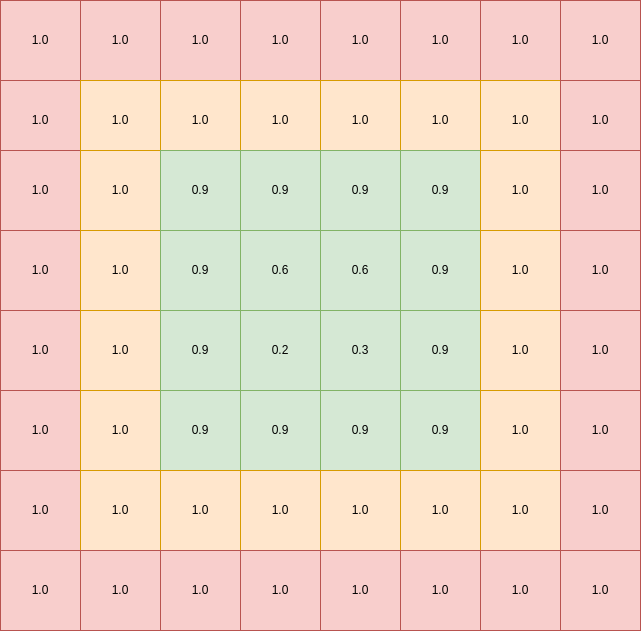
\includegraphics[scale=0.5]{imagenes/Convexidad_buffer.png}
\caption[Visualización de una convexidad a nivel del buffer de profundidad]{Visualización de una convexidad a nivel del buffer de profundidad, en verde los pixeles que forman parte de la convexidad y no marcan la frontera de esta, en naranja los vertices que forman parte de la convexidad y forman la frontera de la convexidad. En rojo los pixeles que no forman parte de la convexidad}

\end{figure}

\section{Visualización y control sobre las transformaciones aplicadas en la convexidad}

\section{Exportación de la malla transformada a un formato de descripción de objetos tridimensionales}

\section{Consideraciones finales y estructura de la implementación}


